%
%  アブストラクトのサンプルファイル (UTF-8)
%
%   Updated: 2016/12/01 Kou Fujimoto (kou-f@mail.dendai.ac.jp)
%   prepared by Takayuki Okuno (t_okuno@ms.kagu.tus.ac.jp)
%
\documentclass[twoside,twocolumn,10pt]{jarticle}  % 2段組の場合
%\documentclass[11pt]{jarticle}   % 1段組の場合
\usepackage{latexsym,amssymb}
%\usepackage[dvips]{graphicx} % epsファイルを使う場合
\usepackage[dvipdfmx]{graphicx}
\usepackage{orsabs-utf8}
\usepackage{amsmath}
% \usepackage{nccmath}
\usepackage{algorithm}
\usepackage{enumerate}
\usepackage[hyphens]{url}
\newcommand{\bm}[1]{{\mbox{\boldmath $#1$}}}
%%%%%%%%%% Title %%%%%%%%%%%%%%%%%%%%%%%%%%%%%%%%%
\title{OpenPNEのソフトウェアエージングに関する研究}
\author{\begin{tabular}{lll@{}ll}
         & 東京都立大学 & *&近藤和希 & KONDO Kazuki \\
        会員 & 東京都立大学 &  &肖霄 & XIAO Xiao
        \end{tabular}}
\date{}
\begin{document}
\maketitle
%%%%%%%%%% ここから本文%%%%%%%%%%%%%%%%%%%%%%%%%%%
\section{序論}
デジタル技術が発展した現代では,私たちの身の回りから宇宙規模のものまでがソフトウェアシステムで構築されており,非常に長時間の連続稼働が必要なものも数多く存在する.
一方で,開発時のソフトウェアテストで得られるバグは,明確に定義された条件下のものであり,リリース前に完全に原因を解決することは難しい.
このような連続稼働による予期しない性能劣化が生じる現象は「ソフトウェアエージング(老化)」と呼ばれる.
% 特に,ソフトウェアエージング関連の障害は,開発の段階で発見し,完全に原因を解決することは難しいものであるとも述べられている\cite{Grottke2007Fightinga}.\par
現代では,特に高可用性が要求される最新のソフトウェアシステムに対する要求が高まり,それらのソフトウェアエージングのリスクを定量的に評価する必要性が高まっている.
% 1990年代初頭から,ソフトウェアエージングに関する広範な研究が行われてきた.
% しかし,ソフトウェアエージングの振舞はソフトウェアシステムの種類によって異なる.
% そのため,ソフトウェアエージングのリスクを評価することは,ソフトウェアシステムの種類ごとに不可欠だと言える.
% 身近なデジタルサービスから社会的な機能を提供する現代のソフトウェアシステムの多くは,伝統的なクライアント/サーバーシステムで構築され様々な種類が存在する.
% いくつかの研究\cite{Grottke2006Analysis}\cite{Alonso2010Adaptive}\cite{Alonso2011Predicting}\cite{Magalhaes2010Prediction}は,これらのシステムを評価している.\par
ソフトウェアエージングのリスクが観測された場合,次に検討すべきはソフトウェア若化手法の検討である.
ソフトウェアエージング関連のバグが蓄積し,それがシステムの性能劣化として現れることを未然に防ぐことが目的である.
% 以下では,障害発生前にシステムを再起動することでソフトウェアエージングによる故障を未然に防ぐという例を挙げて説明する.
% この操作には稼働時間の減少によるユーザーへの影響のコストが発生するため,最適な実行時機を決定することが不可欠である.
% ソフトウェア若化を開始するタイミングを決定する方法は,周期的\cite{Vaidyanathan2005Comprehensive}および非周期的の2つのタイプに分類できる.
% 周期的な手法では,一定間隔でシステムを再起動する必要があるが,非周期的な手法では,特定の基準に基づいてシステムを再起動する必要がある.
% 非周期的手法で広く受け入れられている基準設定の1つは,ソフトウェアシステムのリソースデータから導き出された統計モデルを使用して,経年劣化状態までの時間を予測することである.\par

本研究では,ソフトウェアエージングの研究対象として,SNSシステムの一つであるOpenPNEを選択する.
SNSならではの変動する負荷期間を想定し,監視期間における3種類のメトリクスに着目する.
その結果,比較的低い一定負荷においても,少なくともソフトウェアエージングの潜在可能性を確認できた(暫定).

\section{関連研究と動機}
\subsection{関連研究}
1984年にAdams\cite{Adams1984Optimizing}による継続的なソフトウェア稼働によるパフォーマンスの低下が報告された後,1994年にParnas\cite{Parnas1994Software}によってソフトウェアエージングという用語が最初に使用されたとき,多くの研究者は驚かされ,それ以来広範な研究が行われてきた.
複数のソフトウェアエージングの定義が存在するが,本研究では,Huangら\cite{Huang1995Software}によるシステムの実行時間に焦点を当てたプロセスエージングと呼ばれるソフトウェアエージングの定義に基づき考える.
% Parnas\cite{Parnas1994Software}は,ソフトウェアエージングを次のように定義している.
% 「ソフトウェアエージングには,2つの,非常に異なるタイプがある.
% 1つ目は,製品の所有者が変化するニーズに合わせて製品を変更できなかったことが原因である.
% 2つ目は,行われた変更の結果である.」
% 1年後の1995年,Huangら\cite{Huang1995Software}は,プロセスエージングと呼ばれる,広く受け入れられているソフトウェアエージングの定義を提供した.
% 「プロセスのエージングは,数日から数週間の実行でアプリケーションプロセスが劣化することに関連している」.
% これらの定義の主な違いは,前者がソフトウェアの保守の側面を包含しているのに対し,後者は実行時間に焦点を当てていることである.

Dohiら\cite{Dohi2020Handbook}によると,ソフトウェアエージングの研究は,Threshold-based Approach,Machine learning-based Approach,Measurement-based Approachの3つの手法に分類できる.
本研究では特に,Measurement-based Approachを用いた研究について調査し,多種多様なシステムを対象に行われていることが分かった.
以下,書き方1と2のどちらかで検討中.
1.例として,IBMのクラウドシステム\cite{Sukhwani2017Monitoringa}や画像判定アプリケーションをクラウド環境やエッジ環境にデプロイしたもの\cite{Andrade2020Softwarea}\cite{Andrade2021Memorya}\cite{Andrade2023Comparativea},さらにAndroid OS\cite{Araujo2013Investigative}\cite{Cotroneo2016Software}\cite{Cotroneo2020Comprehensive}やブロックチェーンにまで至る.
2.本分野の研究は,Webアプリケーション\cite{Grottke2006Analysis}\cite{Matias2006Experimental}やクラウドシステム\cite{Sukhwani2017Monitoringa}\cite{Andrade2020Softwarea}\cite{Andrade2021Memorya}\cite{Andrade2023Comparativea}といった多種多様なシステムを対象にし,それぞれのソフトウェアエージングの振舞とその原因を調査している.
% Threshold-based Approachでは,指定された閾値を超える時間を予測する研究や,平均応答時間\cite{Silva2007Using},仮想メモリ使用量\cite{Matias2006Experimental},メモリ使用量\cite{Araujo2011Software}\cite{Avritzer2006Performance}を評価指標として閾値を決定する方法を提案する研究が行われてきた.
% Threshold-based Approachだけでは,ソフトウェアシステムを活性化し若化を行うために最適な時期を見つけるには不十分だが,他の2つのアプローチと組み合わせて使用される.

% Machine learning-based Approachでは,上記の2つのアプローチに機械学習を適用して,精度を高めている\cite{Alonso2010Adaptive}.
% 機械学習の分類を使用して,ソフトウェアエージングによって引き起こされる異常を特定する試みがいくつか行われている\cite{Alonso2011Predicting}.
% Measurement-based Approachでは,Mann-Kendall検定とSenの傾き推定を使用したソフトウェアの経年劣化の検出\cite{Garg1998Methodologya},主成分分析\cite{Cotroneo2010Software}を使用したソフトウェアエージングの識別,ログデータを使用した因子分析など,ソフトウェアエージングの定量化に多くの労力が注がれてきた.
% さらに,いくつかの論文では,ソフトウェアエージングによるリソースの枯渇時間を推定し,エージングに関連する障害を予測している\cite{Chen2018ARFPredictor}.
% 測定するメトリクスの中でも特に,メモリについては「メモリの枯渇に焦点を当てるのは,メモリのTTE(Time To Exhaustion)がコンピュータシステムのリソースの中で最も低く,メモリ管理のバグ(メモリリークなど)が最も顕著なソフトウェアエージングの原因である」と述べられている\cite{Cotroneo2010Softwarea}.
% 以下では,この手法を用いた研究を,対象となるシステムや環境ごとに分類し紹介する.
% クラウド
% まず初めにクラウドシステムに関するものを挙げる.
% Sukhwaniら\cite{Sukhwani2017Monitoringa}は,2017年にIBM独自のクラウドシステムのソフトウェアエージング現象の調査を行い,リソースの枯渇予測やそれを利用した警告システムの搭載を実現した.
% この研究では,彼らは閾値の検討にも取り組んでいる.
% Andradeら\cite{Andrade2020Softwarea}は,2020年に画像判定アプリケーションをクラウド環境とエッジ環境上でそれぞれ長時間運用し,メモリやCPUのリソースを監視し,エージングの動向を比較した.
% さらに2021年には.同じアプリケーションを,パブリッククラウド環境とプライベートクラウド環境で運用し,使用可能メモリの観点から,それぞれのエージングの潜在可能性を指摘した\cite{Andrade2021Memorya}.
% しかし,前者はGoogleデーモンプロセスに,後者はファイルのインデックス作成プロセスというように,それぞれ異なる原因として関連付けた.
% さらに,2023年には2020年の研究の延長として,ユーザー感知メトリクスとして,画像判定アプリケーションの応答時間ではなく,スループット損失に着目した\cite{Andrade2023Comparativea}.
% そこでは,プロセスレベルでの原因分析に取り組むため,メモリ消費量の多い上位6つのプロセスとRSS(Resident Set Size)の相関関係および因果関係の調査を行った.
% なお,因果関係の調査には,時系列データセットの移動エントロピーを分析している.
% % Android OSとブロックチェーン
% Araujo\cite{Araujo2013Investigative}らは,2013年にAndroid OSのソフトウェアエージングを調査するための方法論を提案し,継続的なリソース監視により,メモリリークの検出に成功している.
% さらに,Cotroneo\cite{Cotroneo2016Software}らは2016年に,起動時間LTの遅延現象を,ユーザー感知メトリクスおよびリソースメトリクスの監視を行い相関を調べた.
% その後,彼らは2020年に原因特定のため,ガベージコレクションの遅延現象を探り,javaコンテナのメモリフラッシュによるリジュベネーションの成功にまで研究を広げた\cite{Cotroneo2020Comprehensive}.
% また,peer-to-peerシステムであるブロックチェーンシステムを扱うものもある.添田さんの論文を参考文献に.
\subsection{動機}
本研究では,SNSシステムの一つであるOpenPNE\footnote{https://www.openpne.jp/about/}を対象にMeasurement based Approachを用いて,ソフトウェアエージングの潜在可能性を調査する.
% OpenPNEとは,株式会社手嶋屋が中心となって,OSS方式で開発されてきたSNS構築ソフトウェアである\footnote{https://www.openpne.jp/about/}.
% 開発の敷居が比較的低く,NHK出版やガンホーゲームのファンサイトなど複数の導入事例もあるSNSということで選択した.
% SNSならではの拡張性の高さも備えており,セットアップに関して,多数の文書が提供されていることも後押しになった.
これまでの研究の中で直接的にSNSシステムを対象にしたものは,私たちの知る限りない.
現代のSNSシステムは拡張性も高くユーザー数も莫大であることに伴い,X社のような運営企業にとって,サーバーの運用リスクは高まっているといえる.
% また,SNSシステム独自のアクセス負荷の時系列変化も考えられる\footnote{https://note.fuller-inc.com/n/ne35c0cdba519}.
% そして,機能も非常に複雑で高層的な処理が必要になるため,サーバーのメトリクス(CPUやメモリ)に代表されるようなSNSに関するあらゆるメトリクスを分析し評価する必要性があると考えられる.
本研究では,これまでの研究でも採用されてきた高/中/低負荷に加え,SNSシステム独自の多種多様な負荷シナリオを検討し,それに応じたソフトウェアエージングの調査を行う.
% そのため,現実のユーザーの運用とは異なると述べられている論文もある\cite{Andrade2023Comparativea}.
% 負荷シナリオの検討においては,なるべくシンプルでありながら,ソフトウェアエージングを引き出すようなバランスの取れたストレステストの考案が必要であると考えられる\cite{Cotroneo2016Software}.
また,本研究では,Torquatoら\cite{Torquato2018SWAREa}が2018年に,ストレス期間,待期期間,若化期間のそれぞれでリソースの監視を行った研究を参考にし,本研究では監視期間というものを考える.
ただし,本研究では若化期間には踏み込まない.

\section{本研究の実験環境(予備知識)(名検討中)}
\label{preparing}
% \begin{figure}
%   \centering
%   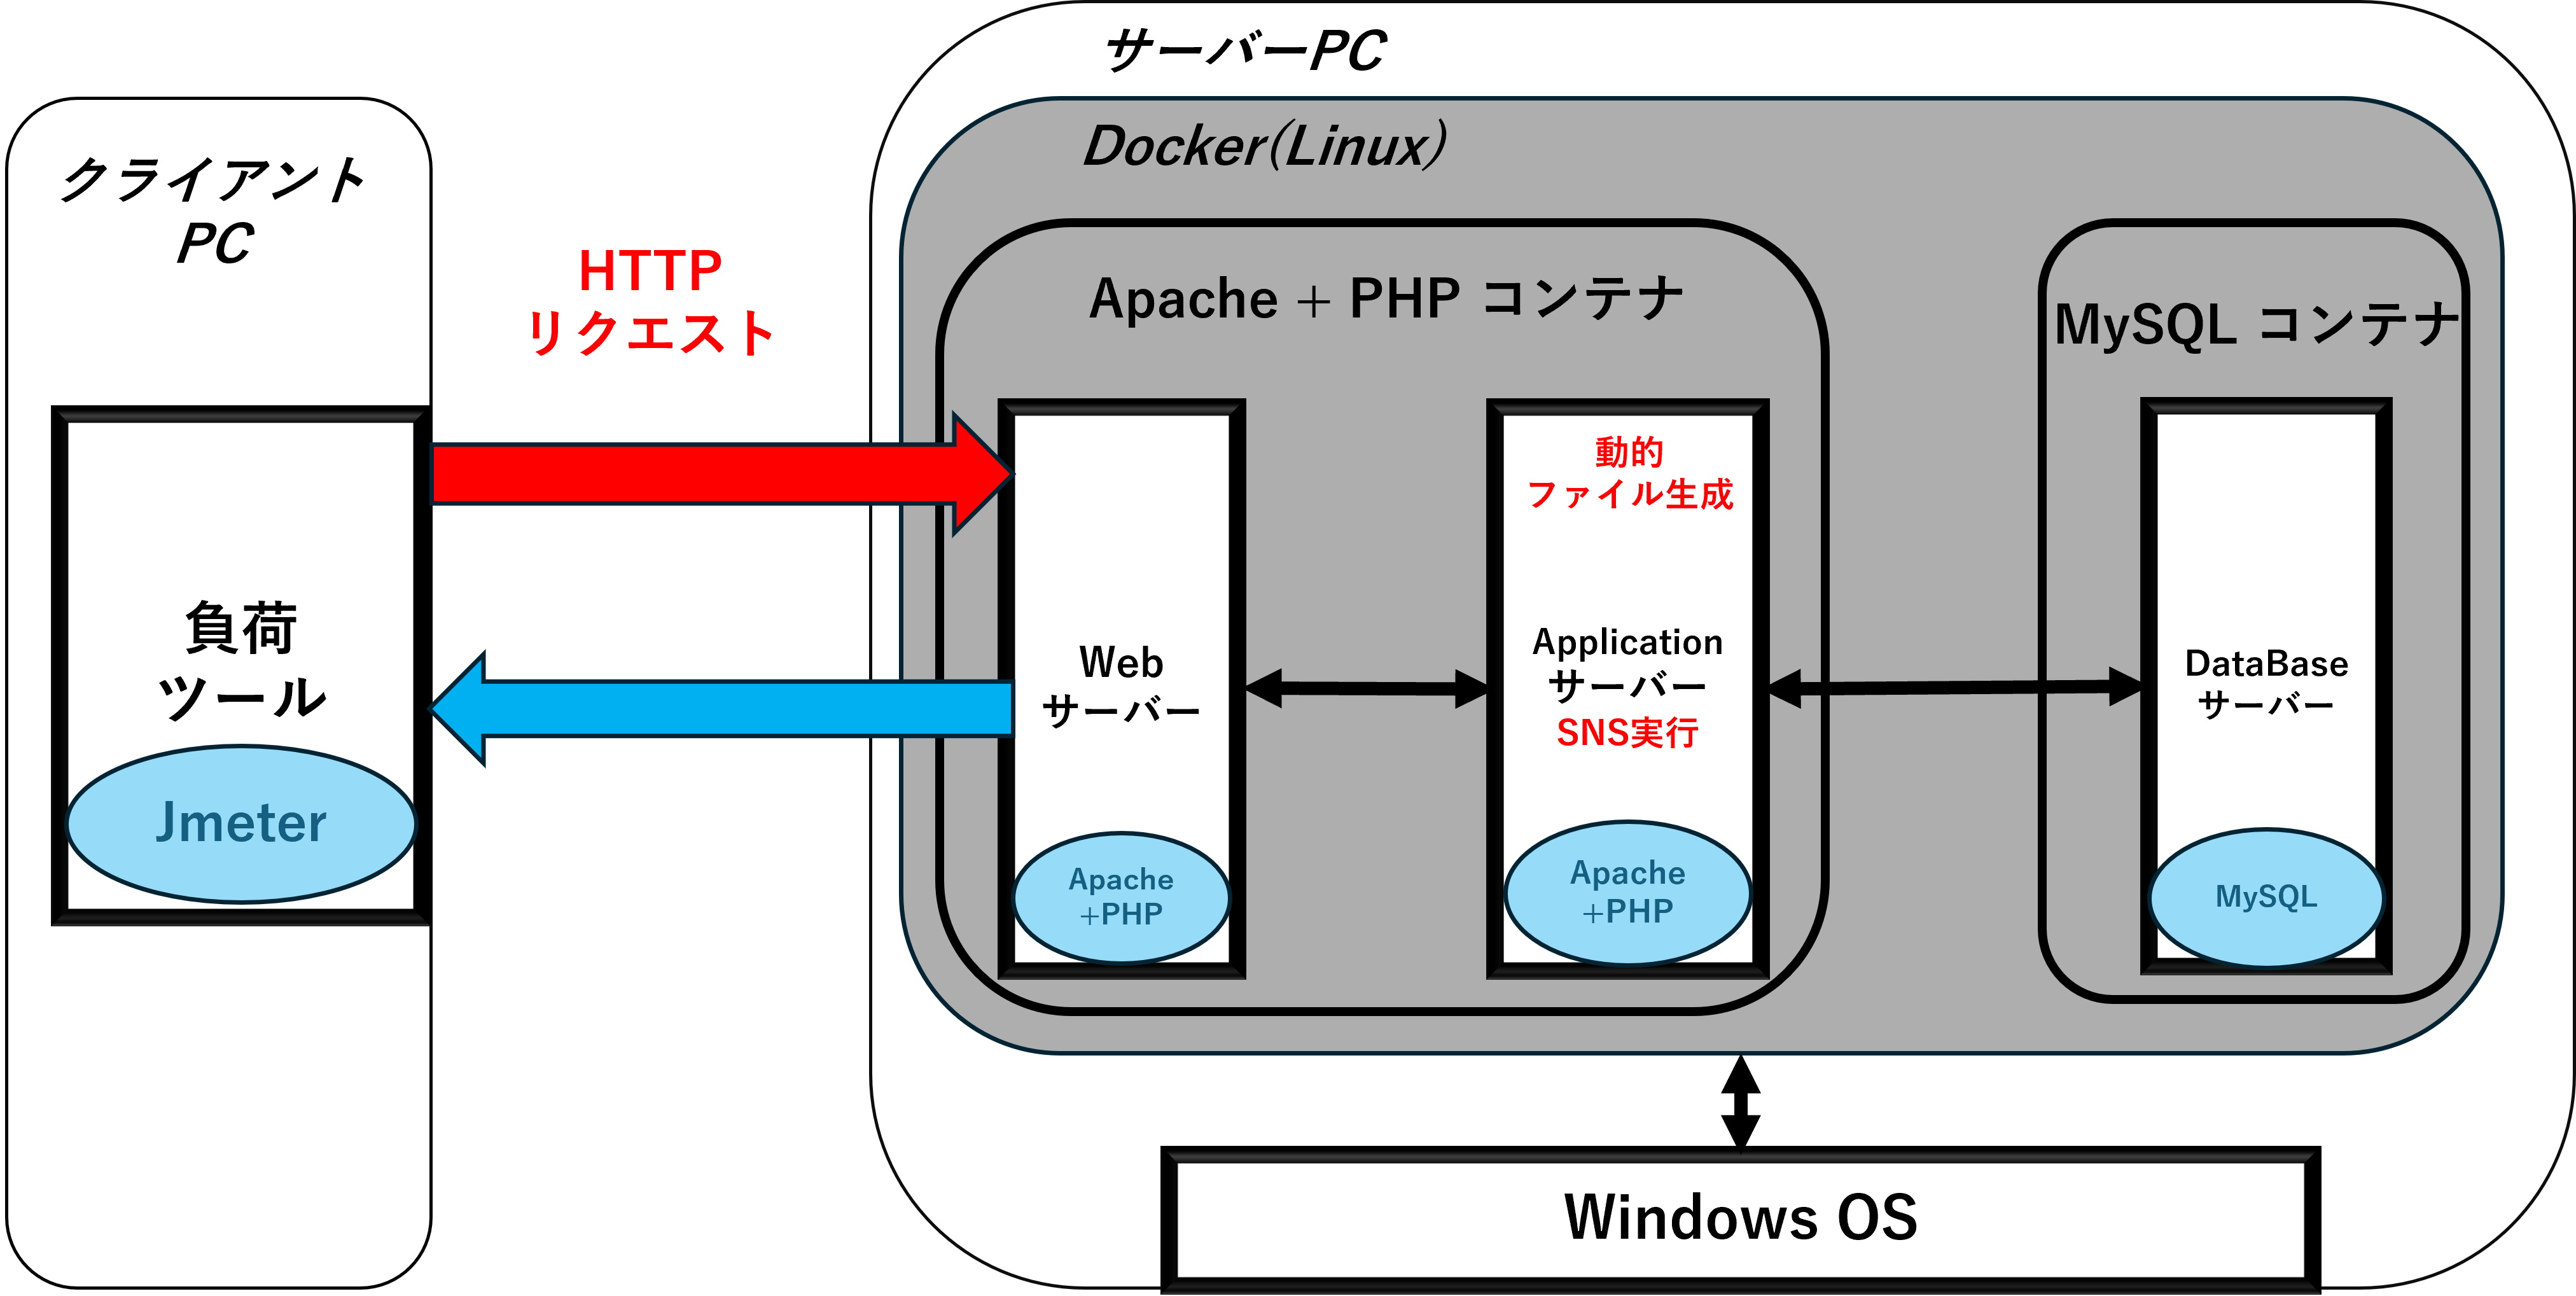
\includegraphics[scale=0.29]{figure/SNS_Docker.png}
%   \vspace{0.05cm}
%   \caption{環境2, fig.3 Environment 2}
%   \label{fig:3}
% \end{figure}

\subsubsection{環境設定}\label{subsec:env2}
※図の記載については検討中.
この環境では,Dockerにより,サーバーPCのOSとOpenPNEの運用環境を隔離している.
また,OpenPNEの環境をDocker上に独立させることでメトリクスをよりクリーンに取得でき,移植性も高い.\
一方で,負荷ツールとの間をLANケーブルでつなぐため,物理的な接続の影響を受けるリスクがある.
% メリット:
% \begin{quote}
%   \begin{itemize}
%   \setlength{\parskip}{0cm} % 段落間
%   \setlength{\itemsep}{0cm} % 項目間
%   \item DockerのホストPCのOSをOpenPNE運用と分離可能.
%   % \item サーバー側への負荷ツールの影響を排除可能.
%   \item SNS環境のみをDocker上に独立させることが可能.
%   \item SNS環境の移植性が高い.
%   \end{itemize}
% \end{quote}

% デメリット:
% \begin{quote}
%  \begin{itemize}
%  \setlength{\parskip}{0cm} % 段落間
%  \setlength{\itemsep}{0cm} % 項目間
%  \item 負荷ツールとの間で物理的な接続の影響を受ける.
%  \end{itemize}
% \end{quote}
% 上の図\ref{fig:3}は物理WindowsデバイスをホストPCとしてDockerでサーバー環境を整えたものである.\par
物理デバイス:\par
\begin{quote}
  \begin{itemize}
  \setlength{\parskip}{0cm} % 段落間
  \setlength{\itemsep}{0cm} % 項目間
  \setlength{\baselineskip}{3pt}
  \item サーバー:HP Z2 mini G9 workstation desktop PC,13th Gen Intel(R)Core(TM) i9-13900 3.00GHz,RAM:16.00GB,Win11 pro,23H2
  \item クライアント:Desktop-7CL98lG,Intel(R) Core(TM) i7-6600U CPU 2.60GHz,RAM:8.00GB,Win10 Enterprise,22H2
  \item LANケーブル
  \end{itemize}
\end{quote}
データ収集:
\begin{quote}
   \begin{itemize}
   \setlength{\parskip}{0cm} % 段落間
   \setlength{\itemsep}{0cm} % 項目間
   \item サーバー側:Docker statsコマンドで取得(CPU使用率,メモリ使用量)
   \item クライアント側:Jmeter(リクエストエラー率※以下エラー率と表記)
   \end{itemize}
\end{quote}

\section{実験}
\subsection{シナリオ1:一定負荷}\label{subsec:load1}
本節では,一定負荷によるエージングの影響の調査を行うが,本環境のサーバー性能調査も兼ねている.
現実の状況において,定常状態に相当すると考えている.

\begin{table}[h]
  \centering
  \caption{エラー率と推定RPS:error rate and estimated RPS(有効数字2桁)}
  \label{tab:rps}
  \begin{tabular}{cccc}
      \hline \hline
      RPS & error rate[\%] & estimated RPS & Risk of SA\\ \hline
      10 & 0.87 & - & 〇 \\ \hline
      30 & 56.51 & 13.5 & ×\\ \hline
      50 & 72.75 & 13.63 & 〇 \\ \hline
      70 & 80.20 & 15.33 & × \\ \hline \hline
      % 90 & x & x & x \\ \hline \hline
      Avg & - & 14.15  & -\\ \hline
  \end{tabular}
\end{table}

表\ref{tab:rps}は,複数の一定負荷シナリオのエラー率,およびそれらの値から推定できるRPSを示したものである.
この結果から,本環境の耐久RPSは14.15RPSであると推定する.
また,メモリ使用量については,Mann-Kendall検定とSenの傾き推定の結果から,少なくとも10RPSと50RPSでソフトウェアエージングのリスクが認められた.

\subsection{シナリオ2:増加負荷(監視期間2H)}
\ref{subsec:load1}の結果より,1~15RPSの増加変動を行い,バズ現象を想定する.
対照実験として,5,10,15RPSの一定負荷と比較し,監視期間における各メトリクスの変動に着目し,ソフトウェアエージングの影響の差異に着目する.
\begin{figure}[H]
  \begin{tabular}{rrr}
      \begin{minipage}{.164\textwidth}
          \centering
          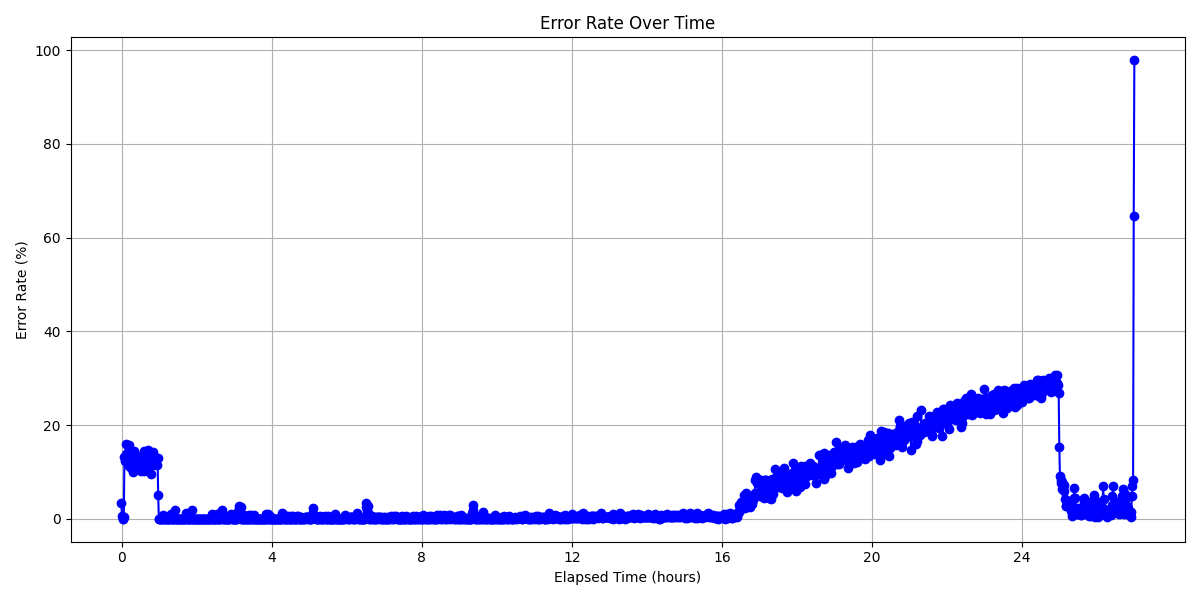
\includegraphics[width=1.2\linewidth]{figures/8core_1_15rps_error_rate.png}
          \caption{エラー率}
          \label{f1}
      \end{minipage}
      \begin{minipage}{.164\textwidth}
          \centering
          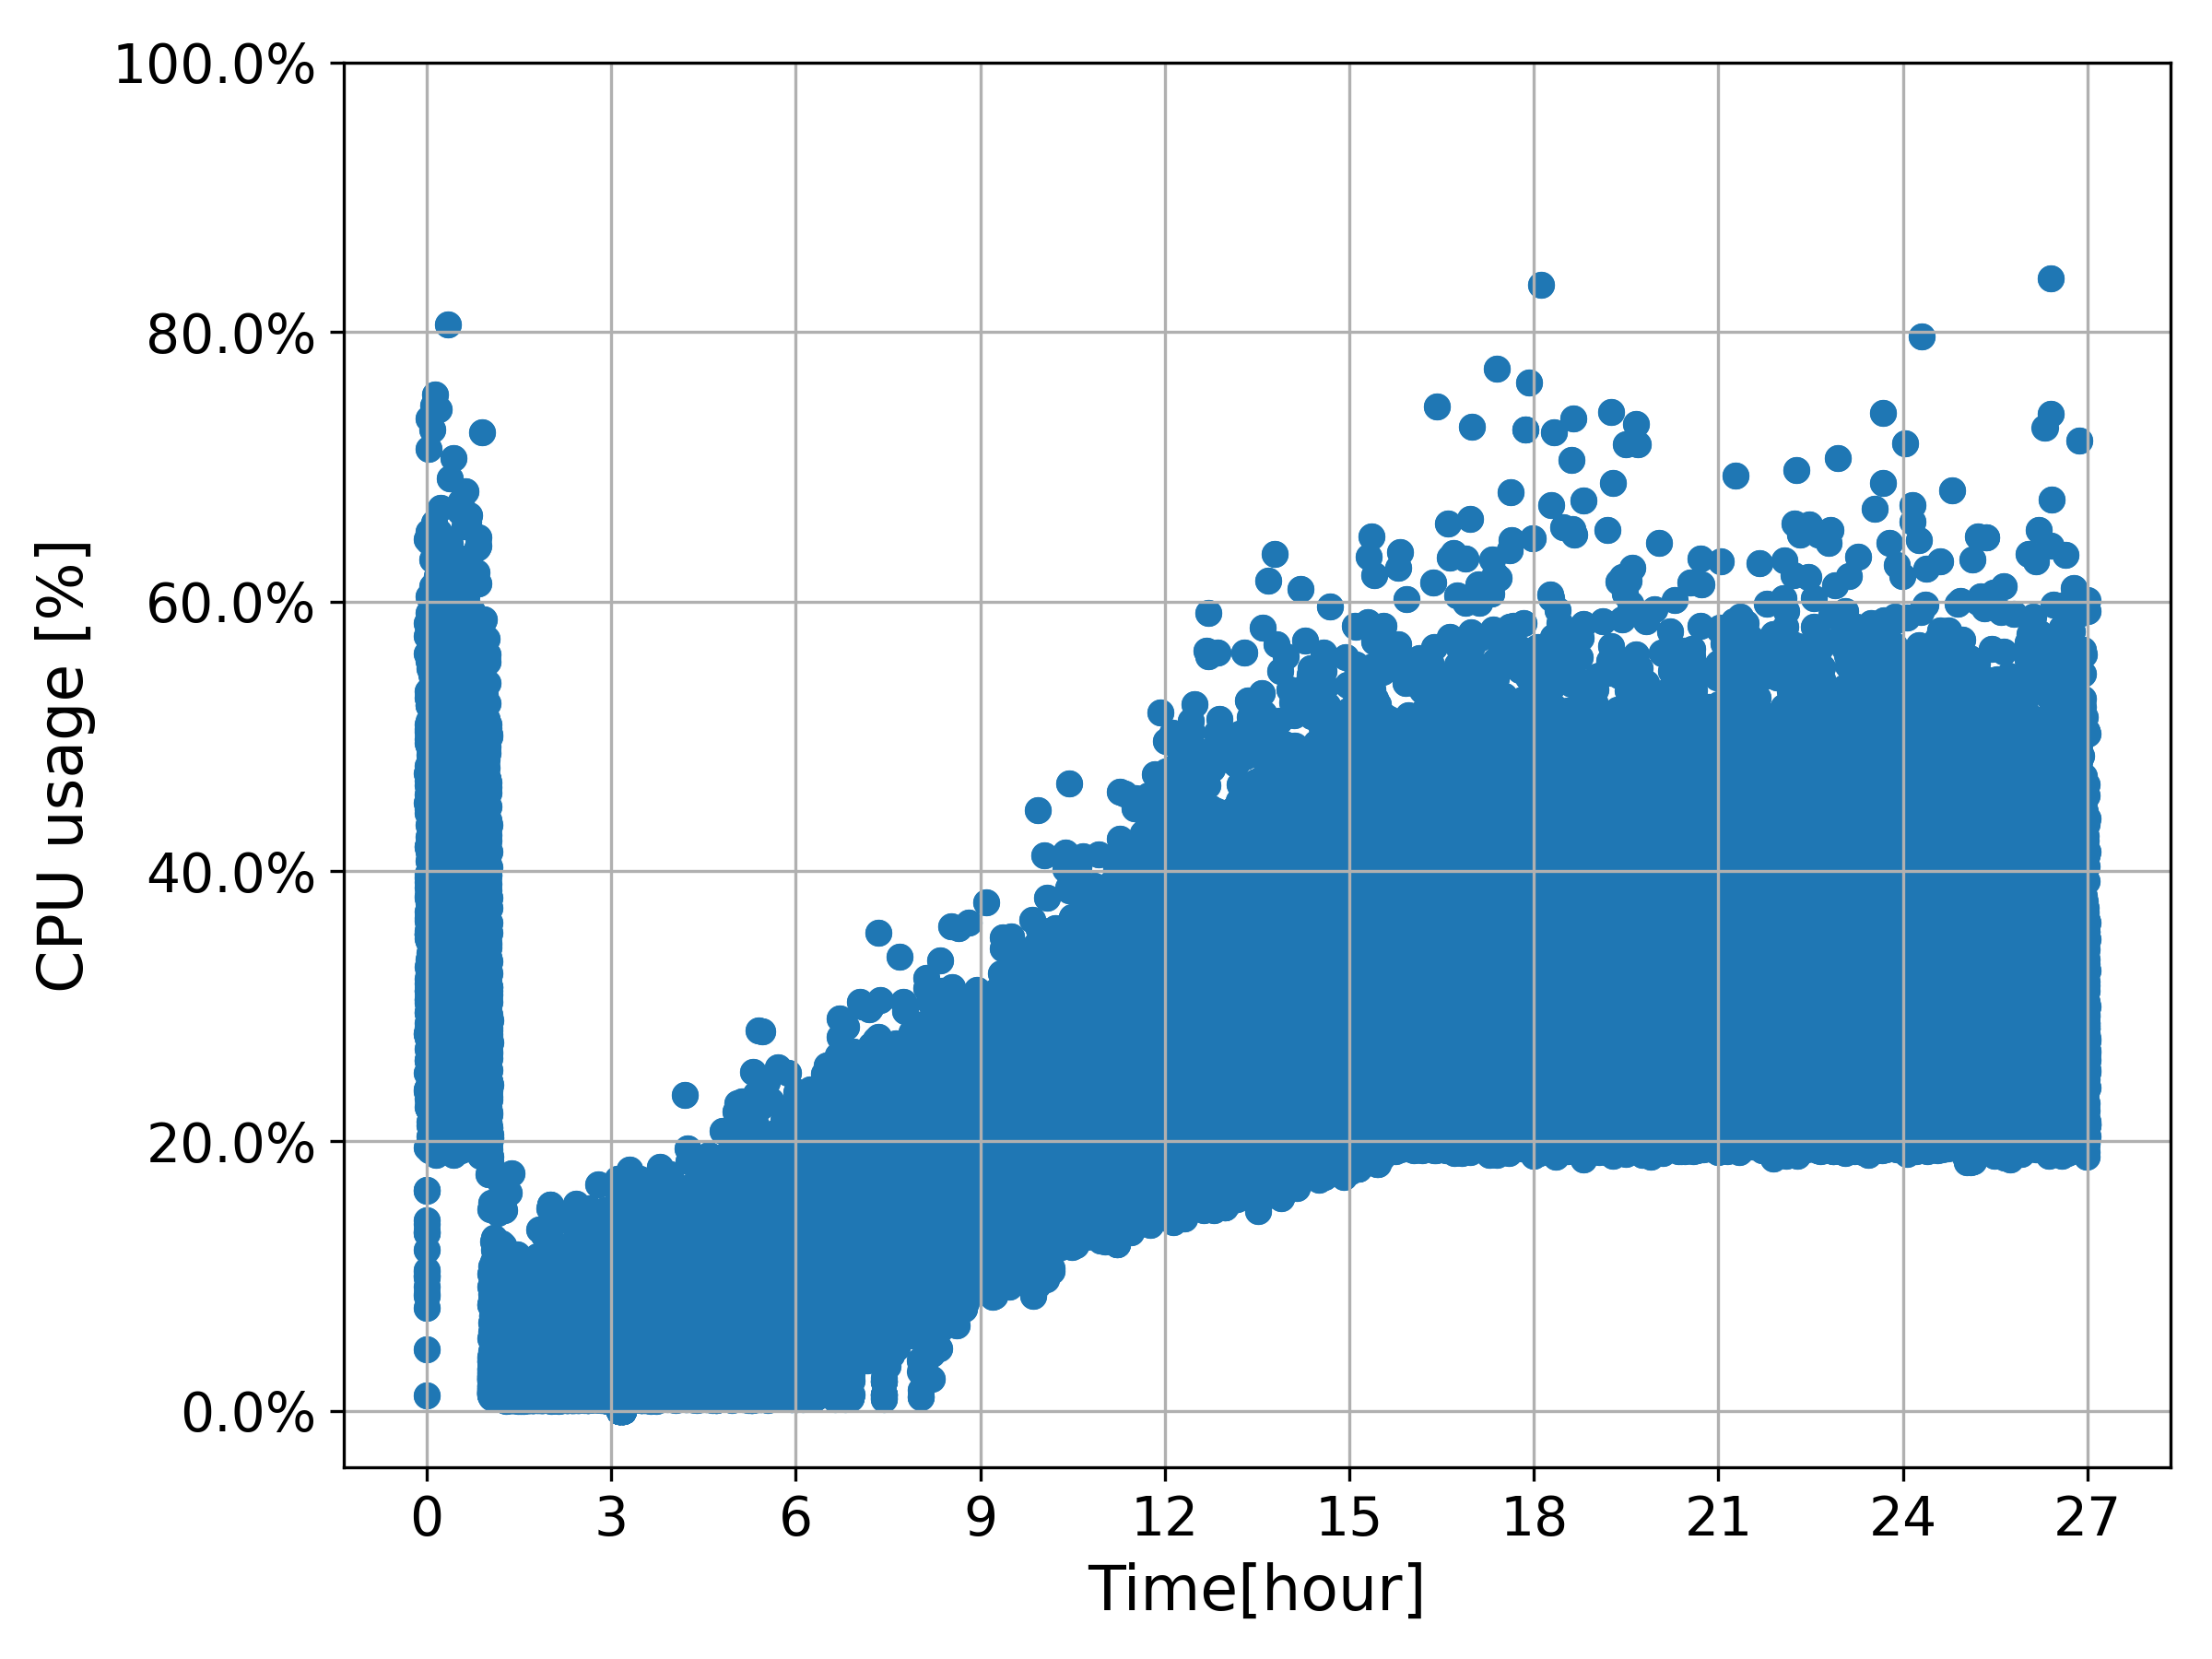
\includegraphics[width=1.0\linewidth]{figures/8core_1_15rps_increase_cpu.png}
          \caption{CPU使用率}
          \label{f2}
      \end{minipage}
      \begin{minipage}{.164\textwidth}
          \centering
          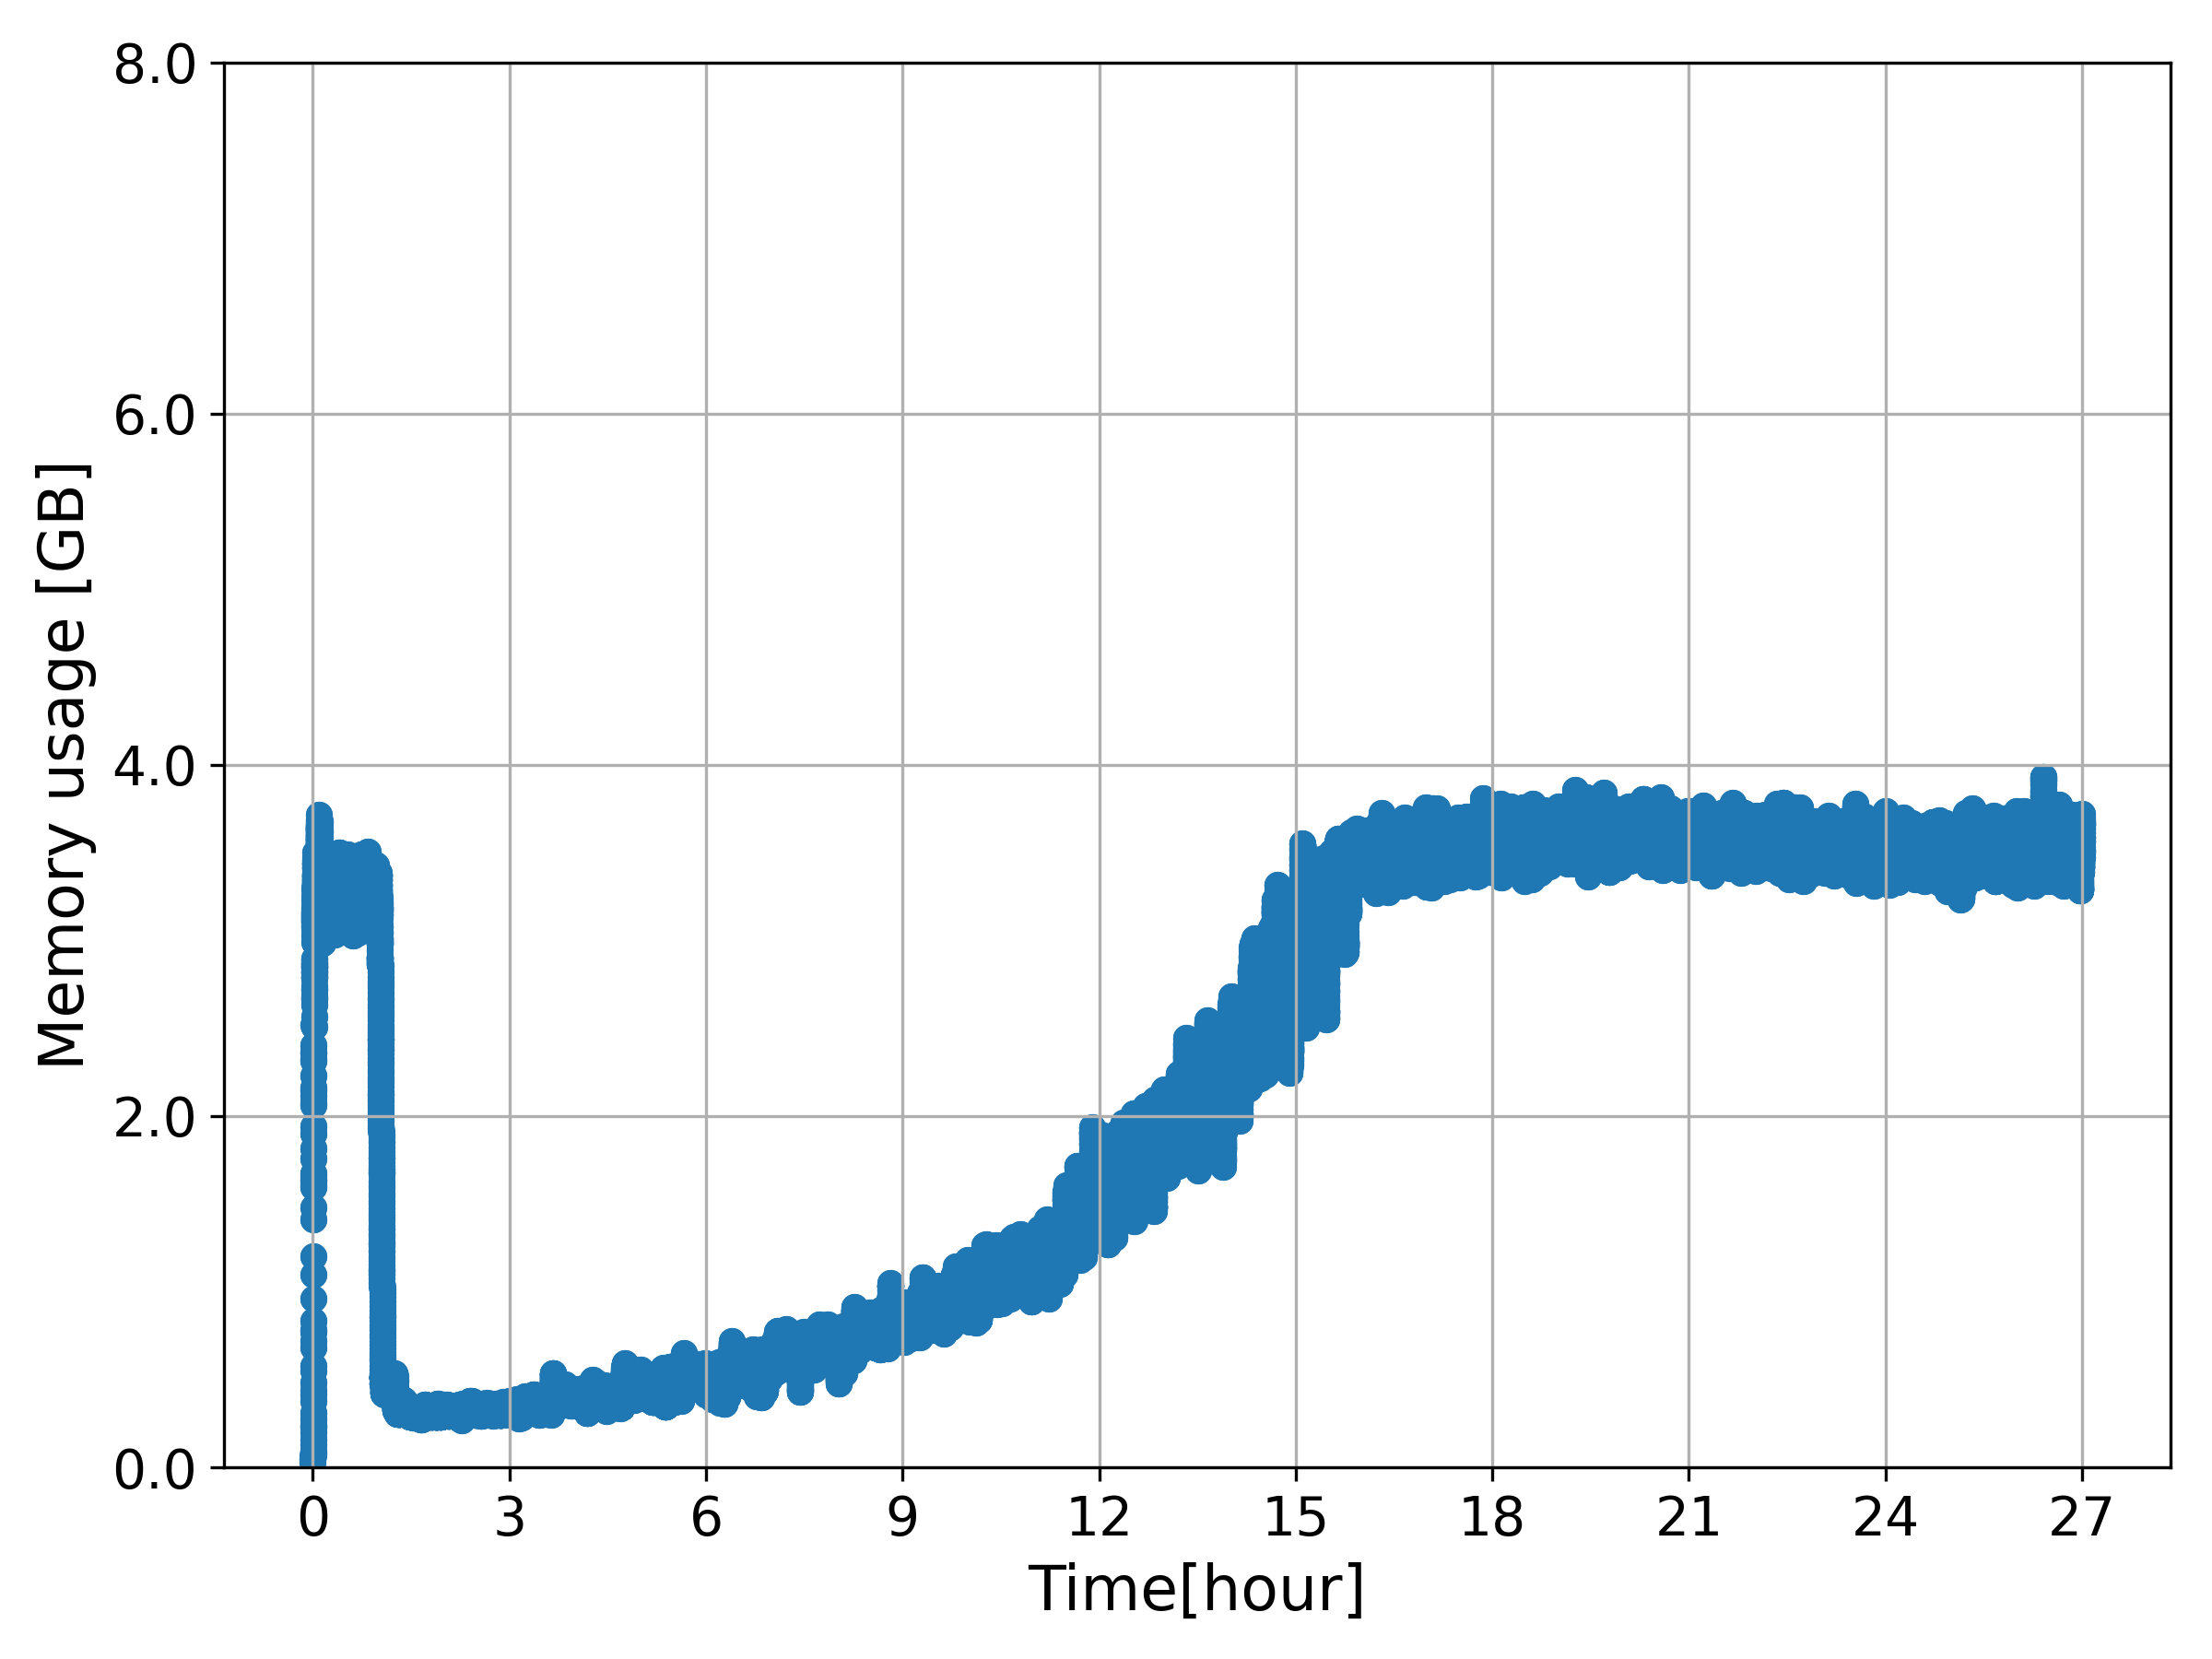
\includegraphics[width=1.0\linewidth]{figures/8core_1_15rps_increase_mem.png}
          \caption{メモリ使用量}
          \label{f3}
      \end{minipage}
  \end{tabular}
\end{figure}

図\ref{f1},\ref{f2},\ref{f3}は,1~15RPSの増加負荷における各メトリクスの時系列変化である.
スレッド立ち上げ期間は負荷の大きさから各メトリクスが比較的高い値を示している.
増加負荷の期間については,増加に伴い,全メトリクスが増加していることが分かる.
特に,エラー率については,RPSが10RPS程度に至る15時間ごろから極端に増加しており,推定RPSよりも低い負荷の段階でエラーを生じた.
一方で,他二つのメトリクスについては,その時間帯までは増加傾向にあったが,それ以降は極端な増加は少なくとも見られない.
これがソフトウェアエージングによる影響かどうかは現時点では判断できない.
また,着目したいのは,負荷後2時間のメトリクスの推移である.
以降については,追加実験の結果が出てから.

\section{結論と今後の展望}
結論については結果がそろってから.\par
本研究では,比較的シンプルなSNSの設定で行ったが,より高度な拡張機能を有したものにすべきといえる.
近年では,序論や関連研究でも述べたようにSNSだけでなく,多くのWebサーバーは,クラウド環境に用意されている.
そのため,今後SNSをクラウド環境にデプロイするなどして,大規模でより現実な負荷テストを行うことが望ましいと言える.
また,本研究ではソフトウェア若化手法についての検討を行っていない.
再起動やガベージコレクションの管理などの代表的な若化手法を,いつ実行すべきかを検討する必要がある.


%%%%%%%%% ここから参考文献 %%%%%%%%%%%%%%%%%%%%%%%
\begin{thebibliography}{5}
  \setlength\itemsep{0.5zh}%←ここの数値を調整(行間のつまり具合)
  \setlength\baselineskip{9pt}
  \textwidth 5pt
  \vskip\baselineskip
  \setlength\baselineskip{6pt}%←ここの数値を調整(追加)(文字の大きさ)
  \bibitem{Adams1984Optimizing}
  Adams, N.Edward, “Optimizing Preventive Service of Software Products,” IBM Journal of Research and Development, vol. 28, no. 1, pp. 2-14, 1984.

  \bibitem{Parnas1994Software}
  D.L.Parnas, “Proceedings of the 16th International Conference on Software Engineering (ICSE1994),” Software aging, pp. 279-287, 1994.

  \bibitem{Huang1995Software}
  Y.Huang, C.Kintala, N.Kolettis and N.D.Fulton, “Software Rejuvenation: Analysis, Module and Applications,” 25th International Symposium on Fault-Tolerant Computing(FTCS1995), pp. 381-390, 1995.

  \bibitem{Dohi2020Handbook}
  T.Dohi, K.Trivedi and A.Avritzer, “Handbook of Software Aging and Rejuvenation,” WORLD SCIENTIFIC, pp. 73-90, 2020.

  \bibitem{Torquato2018SWAREa}
  M.Torquato, Araujo, Matheus, Jean, I.M.Umesh, and P.Maciel, “SWARE: A Methodology for Software Aging and Rejuvenation Experiments,” Journal of Information Systems Engineering \& Management vol. 3, 2018.

\end{thebibliography}
%%%%%%%%%%%%%%%%%%%%%%%%%%%%%%%%%%%%%%%%%%%%%%%%%%
\end{document}